\chapter{The Quest for a Quantum Computer}
Before delving into the question of how we might build a quantum computer, it is worth taking a step
back and exploring the question of what brought us as a scientific community to the point where
it is seen as a priority to build one. The answer to that requires us to delve briefly into
the world of computational complexity theory, and to examine what it means to solve problems "efficiently".
Although the genesis of computation can be traced back to pioneering works by people such as Charles Babbage
and Ada Lovelace in the early 1800's~\cite{Bowden:1953:FTS:1102044}, it was not until the early 1900's that
machines we might recognize as computers were constructed. Based on delicate vacuum tubes, mechanical relays
and often taking up full rooms, their inherent fragility and bugginess posed formidable obstacles to scaling. 
It was not until the mid-1900's that the field took off with two pivotal discoveries. The first
was the construction of the first transistor in 1947, credited to Bardeen, Brittain and Schockley and for which
they were awarded the Nobel prize in 1956~\cite{nobel1956}. This was followed by the creation of integrated circuits by Jack Kilby
in 1959, for which he was awarded the Nobel prize in the year 2000~\cite{nobel2000}. With these two inventions, a remarkable 
surge in computational power occurred. This surge is embodied in Moore's law, which described an annual
doubling in the number of transistors that it would be possible to fit on a single integrated circuit~\cite{4785860}.
And with this doubling came an exponential growth in the computation power that we had available to us.

Along with this growth came an obvious question. What exactly can these computers do? What sorts of
problems will we be able to solve with our ever-growing bundle of transistors? To do this, we need to
think about how many steps it takes to run various algorithms. Take for example the question of looking
for a single item $x_T$, in a list $L = \{x_0, x_1, ..., x_n\}$ with $n$ items in it. Assuming the list
is in an unknown order, to find the location of the item $x_T$, we need to look at each item in the list
in turn. If the length of the list were doubled to $2n$ items, it would take twice as many comparisons to
look through the list. Tripled would be three times. The amount of time it takes to find an item in the
list is \emph{linear} in the length of the list. We can write this mathematically using big$\mathcal{O}$ 
notation: searching for an item in a list is $\mathcal{O}(n)$. 

What about a slightly more complicated problem. What if we want to check whether any item $x_i$ appears
in the list twice? To run this algorithm, we can run the above algorithm for each item in the list, setting the
target to $x_T = x_0$, then $x_T = x_1$ and so forth, and checking whether we find the item two or more
times. So for $n$ items in the list, we run through the list $n$ times, so the number of steps to run
the algorithm scales as $\mathcal{O}(n^2)$. That is, if the length of the list is doubled, it takes
four times as long, so the scaling is \emph{quadratic}.
In this way, we can classify algorithms into various complexity classes. For example, sorting a list
of $n$ items is in the best case $\mathcal{O}(n \log(n))$. Solving the travelling salesman problem (TSP) is
$\mathcal{O}(n^2 2^n)$. More generally, we can group problems into those that have at worst a polynomial
complexity, i.e. $\mathcal{O}\left(f(n)\right)$ where $f(n)$ is a polynomial. These problems are 
in the complexity class \cc{P} (for polynomial), and are said to be \textbf{efficiently} computable.
Those problems that have a difficulty that grows faster than a polynomial in the size of the problem, 
for example, problems whose complexity grows exponentially, are said to be inefficient to compute.

Of course, you might say, well what sort of operations do we allow our computers to do in a single step?
If I say that my computer can solve the TSP in a single step, then the complexity reduces trivially to
$\mathcal{O}(1)$. The answer is not so trivial --- it is limited by the laws of physics. What sorts
of computation do they allow? To answer this question, Alan Turing and Alonzo Church came up with the notion of 
the Turing Machine, a universal model for a computational device, and with it stated the Church-Turing 
hypothesis:

\begin{displayquote}[\cite{turingthesis}]
  "a function is effectively calculable if its values can be found by some purely mechanical process". 
  We may take this literally, understanding that by a purely mechanical process one which could be carried out by a machine.
\end{displayquote}

To paraphrase, this stated that anything a Turing machine could do, a computer could do too, and anything
it \emph{can't} do, no computer can. It wasn't long before this was extended to the strong Church-Turing
hypothesis, which states \textquote[\cite{kaye2007an}]{A probabilistic Turing machine can efficiently simulate any 
realistic model of computation}.
\footnote{In fact, we have to make an addition to the class of algorithms that a Turing machine can run efficiently
 due to the discovery of probabilistic algorithms, which can solve some problems with $> 2/3$ chance in
 polynomial time. By running these algorithms repeatedly, we can solve problems to within an arbitrarily small 
 error $\epsilon$. This class of efficiently computable functions is called bounded-error probabilistic polynomial (\cc{BPP}).}
Note the addition of the term \textbf{efficiently}. This implies that for any
operation we could add to any hypothetical computer, we can get at most a polynomial speedup. Since
a polynomial $P(n)$ divided by another polynomial $Q(n)$ is still a polynomial, and anything that grows faster
than a polynomial $E(n)$ divided by a polynomial $Q(n)$ still grows faster than a polynomial, we have
a universal definition for problems that are efficient to solve and those that aren't.
\footnote{Of course, since we're continually coming up with better algorithms to solve hard problems,
the set of algorithms that are efficient to solve seems to keep growing!}


\begin{figure}
  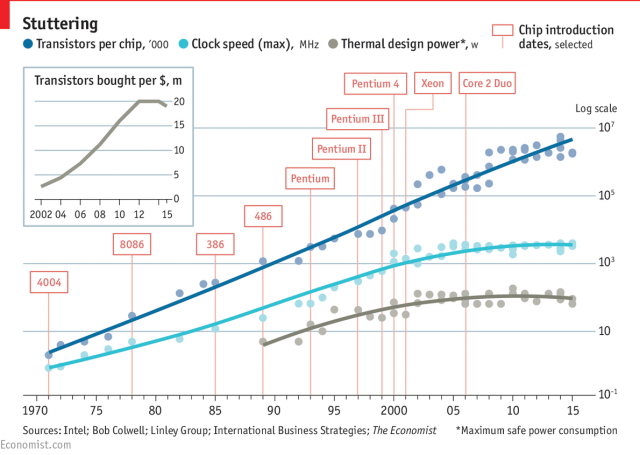
\includegraphics[width=0.7\linewidth]{MooresLaw}
  \caption[Moore's Law and the end of exponential scaling]
  {Graph of the number of transistors per chip, their clock speed, and their
  thermal design power plotted on a log scale against time. Although the number of transistors per chip
  continues to grow exponentially, the clock speed and power per chip have plateaued in the early 2000s.
  Reproduced with permission from~\cite{cross_2016}.}
  \label{fig:mooreslaw}
\end{figure}

So we've established what sorts of problems a computer can solve efficiently, and we've also noted the
exponential growth in the number of transistors on a chip. As long as both of these facts remain true, we
should only have to wait a few years before our computers become twice as powerful and problems that were
previously intractable fall within our grasp. Unfortunately, any exponential scaling must eventually fail,
and so it was for ICs for two key reasons: power and transistor size. As we made our transistors smaller,
we stopped seeing a concomitant efficiency increase, and all of a sudden, the power density of our ICs 
became a limiting factor. To halt this increase, we had to reduce power dissipation, and the
only way we saw how was by capping the speed of our computers, which we can see in figure~\ref{fig:mooreslaw} 
has plateaued since the early 2000s. Moreover, the smaller our transistors became, the more costly they became 
to make. Even Moore's law, which has stubbornly held past the expectations of most scientists, must eventually
end as we bump up against the sizes of atoms. It seems unlikely that there is much room below Samsung's 
recently announced \SI{3}{\nano\meter} node, so if we want to bring more problems into the fold of the
possible, it seems like the strong Church-Turing hypothesis must give.

It was in this context that Feynmann gave his seminal address, noting that as far as we can tell, simulating
quantum systems falls outside of the set of problems that are efficient on classical computers\cite{Feynman1982}. 
However, as long as we can manipulate quantum systems, we should also be able to set up a "quantum
simulator" to see how a quantum system behaves. If this turned out to be the case, then the strong 
Church-Turing hypothesis would be violated!\footnote{Despite this violation, as far as we know the original
Church-Turing hypothesis still holds. No previously uncomputable function became computable with the addition
of quantum physics.} Here was nature efficiently simulating a system that as far as we know, a Turing machine 
can't. It was David Deutsch who in 1985 formalized the idea of a quantum Turing machine\cite{doi:10.1098/rspa.1985.0070}, 
and laid out the Deutsch-Church-Turing hypothesis, which as far as we know holds to this day:

\begin{displayquote}
  A quantum Turing machine can efficiently simulate any realistic model of computation.
\end{displayquote}

\begin{figure}
  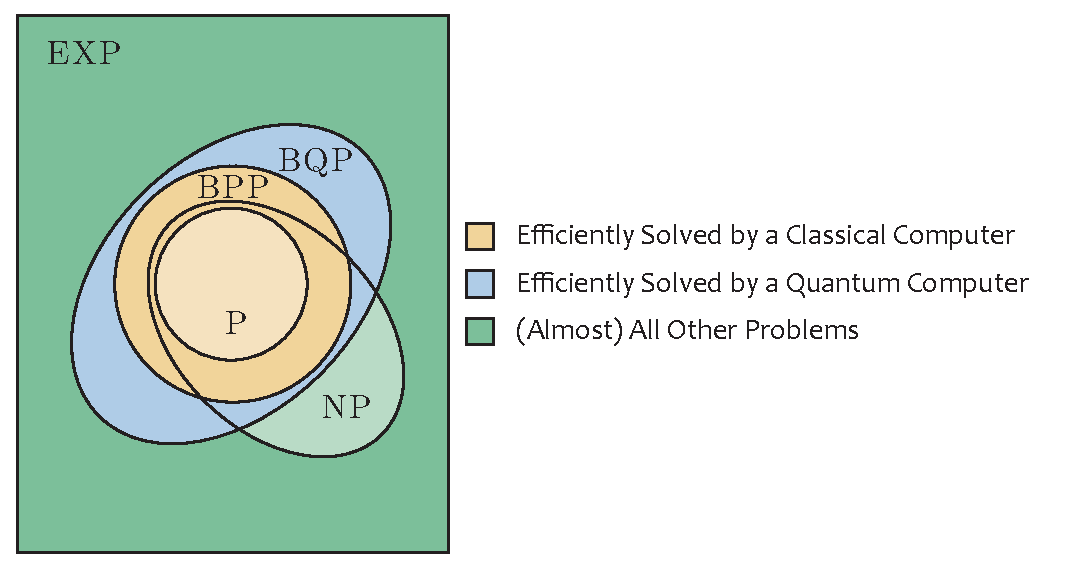
\includegraphics[width=0.85\linewidth]{ComplexityClasses}
  \caption[Relationship between various complexity classes]
  {Relationship between the various complexity classes that we've discussed. The class
  \cc{BPP} includes all problems that a classical computer can solve efficiently (including
  everything that can be calculated in polynomial time). \cc{BQP} are all problems a quantum computer can 
  solve efficiently (which includes everything a classical computer can do). Finally, problems that scale exponentially
  with input size, labelled \cc{EXP}, are (almost) all other problems that are computable. The class
  \cc{NP} is also included on this figure as it is one that often comes up in the context of complexity,
  if for no other reason than to emphasize that a quantum computer \emph{cannot} solve all problems in
  this class.}
  \label{fig:complexity}
\end{figure}

With that, we finally define the class of problems that we might be able to solve efficiently if we 
can build a quantum computer --- Bounded-Error Quantum Polynomial-Time or \cc{BQP}. As far as we know,
this class includes interesting problems that a classical computer could not efficiently solve. Problems
such as Shor's algorithm for prime factorization\cite{Shor} or estimating the ground state of molecules with
the Variational Quantum Eigensolver algorithm\cite{ncomms5213} have no known efficient classical algorithm
but could profoundly impact society if they are solvable. It is the promise of solutions to these problems
that drive the search for a quantum computer; however, the challenges of realizing one remain formidable. To close
out our discussion of complexity classes, I've summarized the relationship between complexity classes in 
figure~\ref{fig:complexity}. To emphasize this point, note that although \cc{BQP} is larger than \cc{P}
or \cc{BPP}, it certainly does not enclose all problems, especially those in \cc{EXP}. Although a
quantum computer may offer an exponential speedup on a subset of algorithms, it will not give us an exponential
speedup in the general case.

The remainder of this chapter aims to lay out the fundamentals of quantum computing and how we might realize
them in a semiconductor system. In \textbf{section~\ref{sec:qc}} I go through a quick introduction to the concepts
underlying quantum computation. In \textbf{section~\ref{sec:qcinsm}} I will detail several methods by which we might
realize a qubit in a semiconductor. Finally, in \textbf{section~\ref{sec:arch}} I will examine the architectural
challenges of realizing a useful, scalable quantum computer.

\section{A Quick Introduction to Quantum Computing}
\label{sec:qc}
To build a quantum computer, we start by defining the notion of a quantum bit (qubit), which
serves as the quantum analog to the classical bit. To review, a classical \textbf{bit} is a "piece" of information
that can take either the value 0 or 1. It represents the fundamental unit of computation in digital computers.
We can take individual bits, and combine them to form a \textbf{register}, whose state is defined as 
the state of each bit in the register. For example, two bits can take up to 4 different
values: 00, 01, 10, 11. Three bits can take up to 9 values, and $N$ bits can take up to $2^N$ values. 
By choosing various encodings of values, we can map numbers, letters, and other symbols onto these registers
and perform computations on them. For example, we can map positive integers onto registers using a base-2 number 
system, as in figure~\ref{fig:binary}, or letters using a mapping such as ASCII, which assigns letters to 8-bit registers.
Other mappings exist for negative numbers (such as a mapping called two's complement), numbers with
decimal points (such as IEEE floating point), complex numbers and so forth. 

\begin{figure}
  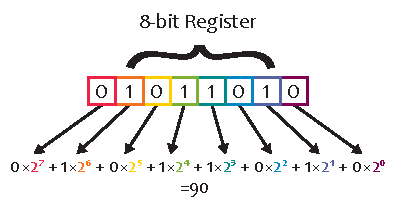
\includegraphics[width=0.75\linewidth]{Binary}
  \caption[Binary Coding]
  {We can encode information in a register in many ways. One encoding for positive numbers is to use a base-2
  positional system, like above, where the binary register \texttt{01011010} is mapped to the number 90.}
  \label{fig:binary}
\end{figure}

\subsubsection{The Qubit}
A \textbf{qubit} is similar to a bit in that it has two states, $\ket{0}$ and $\ket{1}$, except unlike a bit, it is specified
by a 2-dimensional vector, and evolves according to the rules of quantum mechanics. Due to the uniquely quantum
mechanical property of \emph{superposition}, we can no longer write the state of a single qubit (which we will
denote $\psi$) as either $\ket{0}$ or $\ket{1}$. Instead, we must write down the vector sum of the two states,
which we define as follows:
\begin{align}
  \label{eqn:basisstates}
  \ket{0} = \svec{1\\0} && \ket{1} = \svec{0\\1}
\end{align}
\begin{equation}
  \ket{\psi} = \alpha \ket{0} + \beta \ket{1} = \svec{\alpha\\\beta}
\end{equation}
where $\alpha$ and $\beta$ are complex numbers. If we were to take a measurement of this quantum state,
rather than getting back the value of this vector sum, we would measure the $\ket{0}$ state with probability
$|\alpha|^2$ and the $\ket{1}$ state with probability $|\beta|^2$. Since probabilities must sum to one, we also
get a normalization condition: $|\alpha|^2 + |\beta|^2 = 1$. The quantities $\alpha$ and $\beta$ are called
probability amplitudes, and they can take both positive and negative complex values
\footnote{Interestingly, the "complex" part of that state is unnessecary to get the extra computing power
  of a quantum computer\cite{doi:10.1142/S0219749913500019}. There's a good reason that quantum mechanics 
  uses complex probability amplitudes\cite{2004quant.ph..1062A}, but if they were real, it turns out
  we can still do computations in \textsc{BQP} efficiently.} 
as long as the sum of their squared magnitudes to one. This gives us the first hint as to why quantum computing
might give us more power than a classical computer: their states can interact in a manner which mirrors
interference!

\begin{figure}
  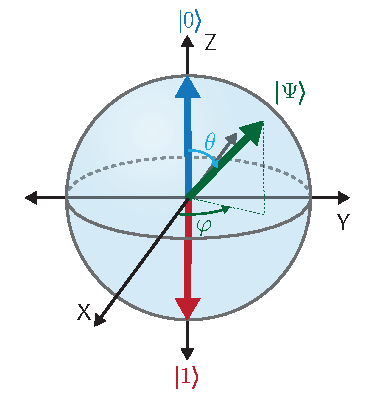
\includegraphics[width=0.5\linewidth]{BlochSphere}
  \caption[The Bloch Sphere representation of a qubit]
  {The state of a qubit can be represented as vector on the surface of a unit sphere. In this description, 
  the state is described by two angles: $\theta$ and $\psi$.}
  \label{fig:bloch}
\end{figure}

Too see how this is true, it's helpful to rewrite the above state in spherical coordinates. First, let's
write $\alpha = r_0e^{-i\varphi_1}$ and $\beta = r_1e^{-i\varphi_2}$. The normalization condition is now
$r_0^2 + r_1^2 = 1$, from which we can make the replacement $r_0 = \cos(\theta/2)$ and $r_1 = \sin(\theta/2)$.
We can also factor out the phase $\varphi_1$ to give:
\begin{equation}
\ket{\psi} = e^{-i\varphi_1}\left(
    \cos\left(\frac{\theta}{2}\right)\ket{0} + e^{-i(\varphi_2 - \varphi_1)}\sin\left(\frac{\theta}{2}\right)\ket{1}
  \right)
\end{equation}
The term $e^{-i\varphi_1}$ is called a global phase factor, and is equivalent to a multiplication by a unit vector,
which it's easy to see makes no difference to the probabilities of any measurement (a fact that will continue to be 
true even when we add more qubits). Another way of saying this is that the important information is encoded in 
the relative phase between the two states. So, let's make the replacement $\phi = \varphi_2 - \varphi_1$ and ignore
the global phase factor, which gives us the state:
\begin{equation}
  \ket{\psi} = \cos\left(\frac{\theta}{2}\right)\ket{0} + e^{-i\phi}\sin\left(\frac{\theta}{2}\right)\ket{1}
\end{equation}
This representation is shown visially in figure~\ref{fig:bloch} and is called the Bloch sphere representation
of a qubit.

Given this description, we can now start to think about what operations on a single qubit might look like.
While on a single bit, the only non-trivial operation we can perform is a flip ($0 \rightarrow 1$ and $1 \rightarrow 0$),
on a qubit we have a whole host of operations that we can perform. The only limits we put on ourselves is that these operations
must leave us on the surface of the Bloch sphere. In other words, after applying an operation, we must still
have a normalized state. From the Bloch representation, you may have already guessed that this means we
can only perform rotations.

Switching back to the 2D vector representation of a qubit, then it's also clear that these operations
must correspond to $2\times2$ matrices. The act of performing an operation corresponds to multiplying
the qubit state by one of these matrices. To ensure that the length of the qubit vector $\ket{\psi}$
remains one at all times, the matrices we can use on our qubit must be unitary. That is, given the matrix $\boldsymbol{M}$,
its complex conjugate transpose $\boldsymbol{M}^\dagger = (\boldsymbol{M^{*}})^\mathrm{T}$ times itself is equal to 
the identity matrix: $\boldsymbol{M}^\dagger\boldsymbol{M} = \boldsymbol{I}$.

Let's define three unit rotation matrices as $\pi$ rotations around the $X, Y, Z$ axes. These have the symbols 
$\sigma_X, \sigma_Y, \sigma_Z$ respectively, and are called the Pauli matrices.
They have the values:
\begin{align}
  \sigma_X = \svec{0&1\\1&0} && \sigma_Y = \svec{0&-i\\i&0} && \sigma_Z = \svec{1&0\\0&-1}
\end{align}

We can build up arbitrary rotations from these unit vectors by taking various powers of these vectors
and multiplying them together. For example to apply a $\pi/2$ rotation around the y-axis applied to the state $\ket{\psi}$
we would perform $\sqrt{\sigma_Y}\ket{\psi}$. \footnote{For those familiar with the rotation operators,
this is more commonly written with a phase factor to make the solution purely real: $R_Y(\tfrac{\theta}{2})
= \exp(-i\pi/4)\sqrt{\sigma_Y}$}
A $2\pi$ rotation around the x-axis would be $\sigma_X\sigma_X\ket{\psi}$. It is possible to generalize this 
to arbitrary rotations, giving us the rotation operators\cite{Nielsen:rot}:
\begin{align}
  R_X(\theta) = e^{-i \theta X/2} = \cos\left(\frac{\theta}{2}\right)\boldsymbol{I} - i \sin\left(\frac{\theta}{2}\right)\sigma_X \\
  R_Y(\theta) = e^{-i \theta Y/2} = \cos\left(\frac{\theta}{2}\right)\boldsymbol{I} - i \sin\left(\frac{\theta}{2}\right)\sigma_Y \\
  R_Z(\theta) = e^{-i \theta Z/2} = \cos\left(\frac{\theta}{2}\right)\boldsymbol{I} - i \sin\left(\frac{\theta}{2}\right)\sigma_Z
\end{align}
These three rotations (and often a global phase factor to simplify our result) are sufficient to express
any single qubit operation. For completeness, we can also define some other gates that often come up in
the context of quantum computation:
\begin{alignat}{4}
    H &=& \frac{1}{\sqrt{2}}\svec{1&1\\1&-1} &=& e^{\tfrac{i\pi}{2}} R_Y\left(\frac{\pi}{2}\right) R_Z(\pi)            &=& \frac{\sigma_X+\sigma_Z}{\sqrt{2}} \\
    T &=& \svec{1&0\\0&e^{\tfrac{i\pi}{4}}}  &=& e^{\tfrac{i\pi}{8}} R_Z\left(\frac{\pi}{4}\right) &=& \sqrt[4]{\sigma_Z} \\
    S &=& \svec{1&0\\0&i}                    &=& e^{\frac{i \pi}{4}} R_Z\left(\frac{\pi}{2}\right) &=& \sqrt{\sigma_Z}
\end{alignat}
These are the Hadamard gate, the T gate (or $\pi/8$ gate)\footnote{The $T$-gate is often 
referred to as the $\pi/8$ gate, even though it represents a $\pi/4$ rotation, a name that is derived from
the phase factor for historical reasons.} and the phase gate respectively.
As is typical, phase factors are usually dropped (something I did not do in the above), hence it is
common to see variations of these equations in the literature. 

As a final example, let's take a detailed look at where interfering probabilities leads to a thoroughly
non-classical result. To start with, let's define two additional states:
\begin{align}
  \ket{+} = \frac{\ket{0} + \ket{1}}{\sqrt{2}} && \ket{-} = \frac{\ket{0} - \ket{1}}{\sqrt{2}}
\end{align}
We can get these states by starting from $\ket{0}$ and rotating $\pi/2$ or $-\pi/2$ around the Y-axis. You can
reasonably easily confirm that they are properly normalized, and that if we were to measure each state, the
probability of measuring a $\ket{0}$ or a $\ket{1}$ are equal for both states: $\mathrm{P}\left(\ket{0}\right) = 
\mathrm{P}\left(\ket{1}\right) = 0.5$. So a direct measurement would be unable to distinguish these two states.
However, if we were to apply the Hadamard gate to each of those two states, we surprisingly end up with two
different outputs:
\begin{align}
  H\ket{+} = \ket{0} && H\ket{-} = \ket{1}
\end{align}
In this case, the complex probability amplitudes can interfere with each other causing the two states to
become distinguishable, something that a classical bit could not replicate. What you see is what you get.

\subsubsection{Multi-Qubit States (Qubit Registers)}
The next additional computational resource that quantum physics gives us is \emph{entanglement}. This 
resource rears it's head when we try to combine multiple qubits into a register. Formally,
we can define entanglement as a correlation between the states of qubits after they have interacted
with each other. Due to this correlation, the state of a qubit that has been entangled with its partner
can no longer be described independently, the states of the two qubits become linked. Perhaps the easiest
way to grok the consequences of this is to give an example of how this correlation might play out.

Let's start with two qubits, one of which starts in the $\ket{+}$ state, the other which starts in
the $\ket{0}$ state. If we were to apply a gate that flips the state of the second qubit if the state of
the first qubit is $\ket{1}$, then we might expect to end up with something like $\ket{+}$ in the second
qubit. If we measure the first qubit and get the result $\ket{0}$, the state of the second qubit must also
be zero, so the state of the second qubit can't have been described by $\ket{+}$. The state of the two
qubits is correlated and depend on each other. The operation we described above is called the 
controlled-NOT ($CNOT$) gate, and creates a state that looks like:
\begin{equation}
  \ket{\psi} = \frac{\ket{00} + \ket{11}}{\sqrt{2}}
\end{equation}
To describe a generalized two-qubit state, we must give coefficients to each possible state the qubits
can take:
\begin{equation}
  \ket{\psi} = \alpha\ket{00} + \beta\ket{01} + \gamma\ket{10} + \delta\ket{11} = 
    \svec{\alpha\\\beta\\\gamma\\\delta}
\end{equation}
So to combine two qubits together, we cannot just list the states of the two qubits one after another,
they are described by the tensor product of the two individual states: $\ket{\psi} = \ket{\psi_1}\otimes\ket{\psi_2}$.
For a three-qubit register, the total number of states we must give coefficients to is 8. For a $N$ qubit
register, the total number of coefficients is $2^N$. Note the distinction between a classical register
and a quantum register, to describe a classical register, we can list the states of the individual
bits one after another, whereas the quantum register requires $2^N$ complex numbers to express fully.

Much like a single qubit, we require new matrices that can operate on quantum registers. As one 
might expect, the size of these matrices is exponential in the number of qubits that we must operate on.
For example, on a two-qubit register, we require a $4 \times 4$ matrix to describe operations. The 
$CNOT$-gate that we used above is defined as:
\begin{equation}
  CNOT = \svec{1&0&0&0\\0&1&0&0\\0&0&0&1\\0&0&1&0}
\end{equation}
Unfortunately, the potential presence of entanglement means applying single or two-qubit gates to a subset
of qubits in the register is no longer a matter of applying a $2 \times 2$ or $4 \times 4$ matrix, we must
construct a $2^N \times 2^N$ matrix and apply that to the full quantum register. This construction is achieved
by taking the Kronecker product of identity matrices and the matrix we want to apply. For example, to apply
a $\sigma_X$ gate to the 2nd qubit in a three-qubit register, we construct the operator as follows:
\begin{equation}
  \sigma_{X,2} = \boldsymbol{I} \otimes \sigma_X \otimes \boldsymbol{I}
\end{equation}

The consequences of the twin effects of superposition and entanglement lead to the extra computational
power of a quantum computer, while also hinting at the difficulty of writing quantum algorithms. As we
can prepare arbitrary superposition states, we can encode an exponentially large
state into a quantum register, for example representing every number between 0 and $2^N-1$ in a $N$ qubit
register, and operate on all of these states in parallel. However, once we measure the register, we end up 
with only one of the possible states in the register (i.e. the state collapses), and the quantum information
that was prepared in the state is lost. Quantum algorithms must, therefore, have three properties to be useful:
\begin{enumerate}
  \item An efficient way of preparing a state. If we want to perform computations on a quantum register 
    storing $2^N$ values, we lose any exponential speedup if we need to load each of these values one-by-one. 
    For example, Shor's algorithm relies on being able to prepare an equal superposition of all states 
    in the register with $N$ single qubit gates\cite{PhysRevA.54.1034}.
  \item Creation of a large entangled state. Without entanglement, a quantum algorithm can be efficiently 
    simulated on a classical computer. The exact role that entanglement plays in computation is not yet known; 
    however, without using it, we know that quantum computers lose their advantage\cite{doi:10.1098/rspa.2002.1097}.
  \item A way of whittling down the quantum state to make the "answer" the likely outcome of any readout. 
    Since coefficients in a quantum register represent probability amplitudes that measurement will yield 
    a given outcome, we can get at most $N$ bits of data per measurement\cite{651037}, as our register 
    immediately collapses into one state upon measurement. To get another value out of the register, 
    we must repeat the whole computation, including loading the state.
\end{enumerate}

% Possible TODO: Circuit notation?

\section{Making Qubits in Semiconductors}
\label{sec:qcinsm}
Having described the basic ideas of quantum computing, our next challenge is to find a physical system that
is able to implement the operations that we discussed above. This problem can be distilled to that
of finding a quantum two-level system that follows a set of criteria that were first laid out by David
DiVincenzo, a criteria that is widely considered to be the standard checklist for any qubit\cite{divincenzo_crit}. They are:
\begin{enumerate}
  \item A scalable physical system with well characterized qubits
  \item The ability to initialize a fiducial qubit state, such that the state of the system is known prior 
    to any quantum operations.
  \item Decoherence time in the qubit subspace that greatly exceeds the gate operation time.
  \item A universal set of quantum gates.
  \item The ability to perform measurements on individual qubits.
\end{enumerate}
Although these criteria set out some requirements for useful qubits, they are certainly not so prescriptive
that there is a dearth of systems that could fulfil them. It is in this context that ion-traps, photonic, 
NMR based qubits, superconducting and semiconductor based qubits are being invevstigated, each with advantages 
and disadvantages for each criterion. Apart from a brief discussion of the scalability prospects of each of these systems
in section~\ref{sec:arch}, I will focus on semiconductor based qubits for the remainder of this thesis. This type
of qubit has the potential to utilize the extroadinary processing capabilities of modern semiconductor manufacturing
although as we shall see, even within this subset of possible qubit systems, there are still many different
choices of two-level subspace. As a result, I will not attempt to comprehensively cover all the variations
of qubit that exist, rather I will focus specifically on two general designs, quantum dots and majorana zero modes,
which in many ways share similar control and readout. This also means that the discussion of physics in this section will
largely be confined to III-V materials, although I will point out that as my thesis is aimed at the general
problem of architecting a quantum computer, many of the results presented may find use outside the subset of physics
I present here. Before we begin a detailed discussion of qubits in semiconductors, let's first take a look 
at the physics that underlie most of these implementations; the 2-dimensional electron gas (2DEG).

\subsection{The 2-Dimensional Electron Gas}
\subsubsection{The Quantum Hall Effect}
\subsubsection{Spin Orbit Interaction}
\subsection{Quantum Dots}
\subsection{Majorana Zero Modes}

\section{Architecture of a Quantum Computer}
\label{sec:arch}
  \subsection{Control Plane}
  \subsection{Readout}